\documentclass{beamer}

\usepackage[utf8]{inputenc}
\usepackage{amsfonts}
\usepackage{amsmath}
\usepackage{xcolor}
\usepackage[noend]{algpseudocode}
\usefonttheme{serif}
\usetheme{Boadilla}
\usecolortheme{seahorse}

\title[Foraging]{Biomimicry of Bacterial Foraging}
\subtitle{for Distributed Optimization and Control}
\author[Passino; Van de Kleut]{
  Kevin M. Passino\inst{1}\\
  Presented by: Alexander Van de Kleut\inst{2}
}
\institute[OST; UW]{\inst{1}
  The Ohio State University\\
  Electrical and Computer Engineering
  \and
  \inst{2}
  University of Waterloo\\
  Centre for Theoretical Neuroscience
}
\date[W20]{IEEE Control Systems Magazine, 2002}

\begin{document}

\frame{\titlepage}

\begin{frame}
\frametitle{Table of Contents}
\tableofcontents
\end{frame}

% Kevin Passino is a professor of Electrical and Computer Engineering at Ohio State University.
% His work covers a broad range of disciplines, from virtual reality for mental health therapy to fuzzy control theory to humanitarian engineering.
% He has done considerable work on biomimicry and swarm intelligence.
% I've included here two selected textbooks he has been a major contributor for: Swarm Stability and Optimization, and Biomimicry for Optimization, Control, and Automation
% The paper I'm presenting today is Passino's second most-cited paper at over 3000 citations.
\section{About the Author}
\begin{frame}
\frametitle{About the Author}
\begin{columns}[T]
  \column{0.5\textwidth}
    \includegraphics<1-2>[scale=2]{assets/kpassino}%
  \column{0.5\textwidth}
    \includegraphics<1>[scale=2]{assets/book1}
    \includegraphics<1>[scale=0.18]{assets/book2}
    \includegraphics<2>[scale=0.3]{assets/citations}
\end{columns}
\end{frame}

\section{Foraging}
\begin{frame}
\frametitle{Foraging}
\textbf{Foraging}
\begin{itemize}
  \item searching for nutrients
  \item avoiding noxious stimuli (toxins, predators, etc)
\end{itemize}
\textbf{Social Foraging}
\begin{itemize}
  \item increases likelihood of finding nutrients
  \item better detection and protection from noxious stimuli
  \item gains can offset cost of food competition
\end{itemize}
\end{frame}

\begin{frame}
\frametitle{Foraging as Optimization}
\textbf{How can we view foraging as an Optimization Process?}
\begin{itemize}
  \item<1-> We have some parameters $\theta$ and a loss function $J(\theta)$ that we want to minimize
  \item<2-> $\theta$ can represent the position of an organism in its environment
  \item<3-> $J$ can represent the concentration of nutrients and noxious stimuli
  \begin{itemize}
    \item smaller values of $J$ = more nutrients, less noxious stimuli
    \item higher values of $J$ = more noxious stimuli, less nutrients
  \end{itemize}
  \item<4-> In general, $J$ and $\theta$ can be arbitrary
  \begin{itemize}
    \item $\theta \in \mathbb{R}^p$
    \item $J: \mathbb{R}^p \to \mathbb{R}$
  \end{itemize}
\end{itemize}
\end{frame}

\section{Building the Algorithm}
\begin{frame}
\frametitle{\textit{E. coli}}
\begin{itemize}
  \item<1-> Model organism
  \begin{itemize}
    \item<1-> Highly studied
    \item<1-> Well-characterized foraging behaviour
    \item<1-> Probably won't feel bad about simplifying its behaviour
  \end{itemize}
  \item<2-> Social organism
  \begin{itemize}
    \item<2-> Secretes signals to attract others nearby
    \item<2-> Encourages ``swarming'' or ``clumping''
  \end{itemize}
\end{itemize}
\end{frame}

\begin{frame}
\frametitle{\textit{\textit{E. coli}} Behaviour}
\begin{itemize}
  \item Swims using left-handed helical flagella (``propellers'')
  \begin{itemize}
    \item \textbf{Tumble}: flagella all rotate clockwise $\to$ pull on cell in all directions $\to$ random movement
    \item \textbf{Run}: flagella all rotate counterclockwise $\to$ flagella form a bundle $\to$ push on cell in one direction $\to$ directed movement
  \end{itemize}
\end{itemize}
\begin{center}
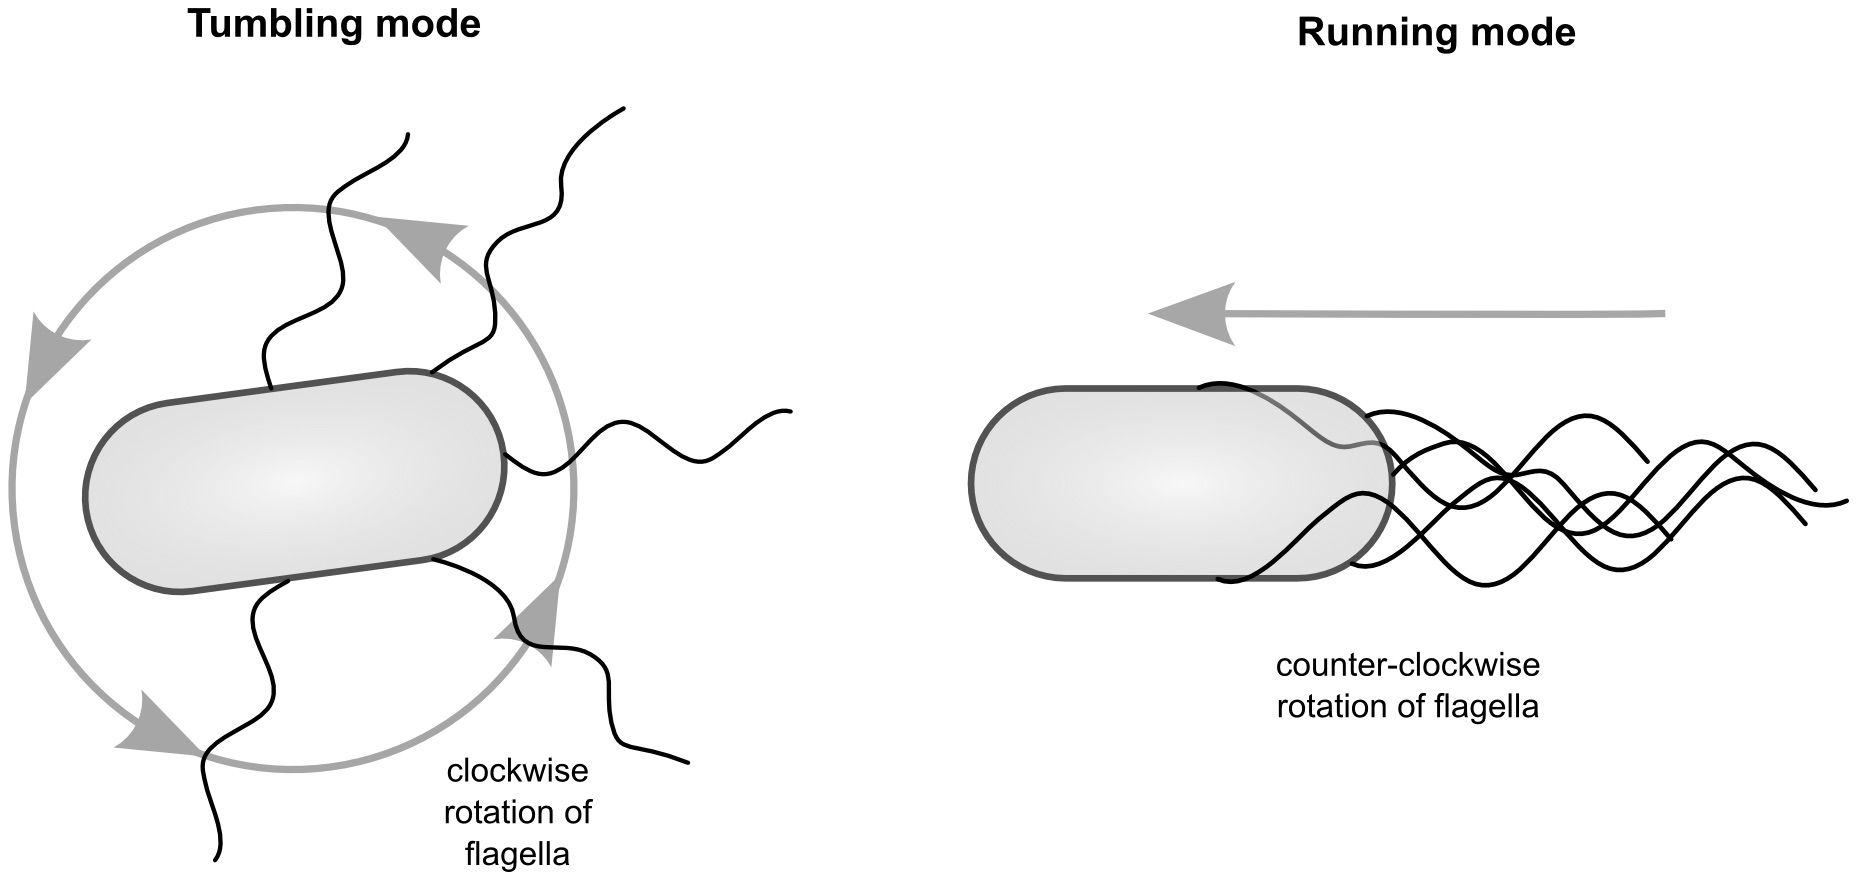
\includegraphics[scale=0.2]{assets/ecoli}
\end{center}
\end{frame}

\begin{frame}
\frametitle{\textit{\textit{E. coli}} Behaviour}
\begin{itemize}
  \item If during a tumble \textit{\textit{E. coli}} swims down a nutrient concentration gradient:
  \begin{itemize}
    \item Prolongs time spent on a run
    \item Continues moving in the same direction
  \end{itemize}
  \item Otherwise:
  \begin{itemize}
    \item Tends to switch to a tumble (search for more)
    \item Moves randomly which searching for more nutrient gradients to exploit
  \end{itemize}
  \item Call a tumble followed by a run a ``chemotaxis step''
\end{itemize}
\end{frame}

\begin{frame}
\frametitle{Algorithm for a Single Bacterium}
\begin{algorithmic}[1]
\For {$j \gets 1 \dots N_c $}:
  \State $\phi \sim S^p$
  \State $\theta \gets \theta + c \phi$
  \While {$J(\theta + c \phi) < J(\theta)$}:
    \State $\theta \gets \theta + c \phi$
  \EndWhile
\EndFor
\end{algorithmic}
\begin{itemize}
  \item $\theta$: $p$-dimensional vector (randomly initialized)
  \item $N_c$: number of chemotaxis steps
  \item $\phi \sim S^p$: a random $p$-dimensional unit vector
  \item $c$: a step-size
\end{itemize}
\end{frame}

\begin{frame}
\frametitle{Loss Function to Optimize}
\begin{center}
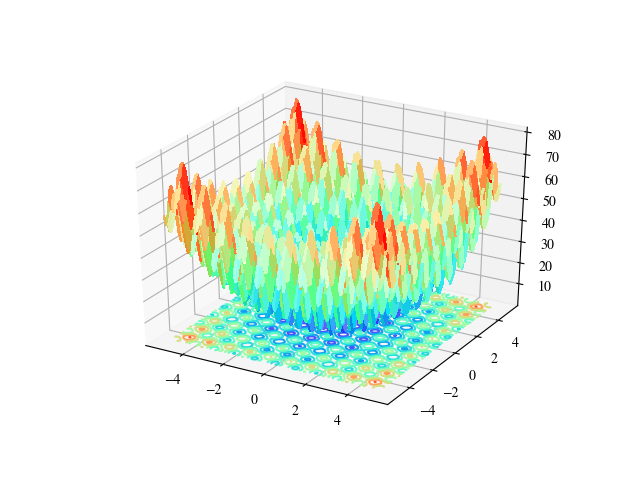
\includegraphics[scale=0.5]{assets/rastrigin}
$$J(\theta) = An + \sum_{i=1}^n \left( x_i^2 - A \cos(2 \pi x_i) \right)$$
\end{center}
\end{frame}

\begin{frame}
\frametitle{Results of Single Bacterium}
\begin{columns}[T]
  \column{0.5\textwidth}
    \begin{center}
      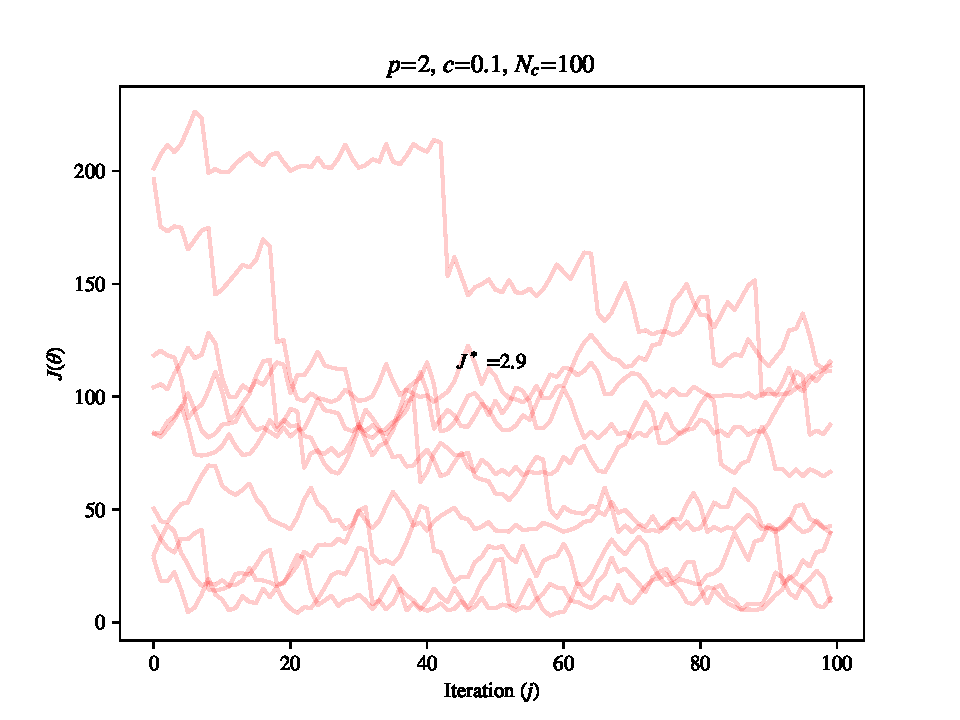
\includegraphics[scale=0.3]{assets/rastrigin_J}
      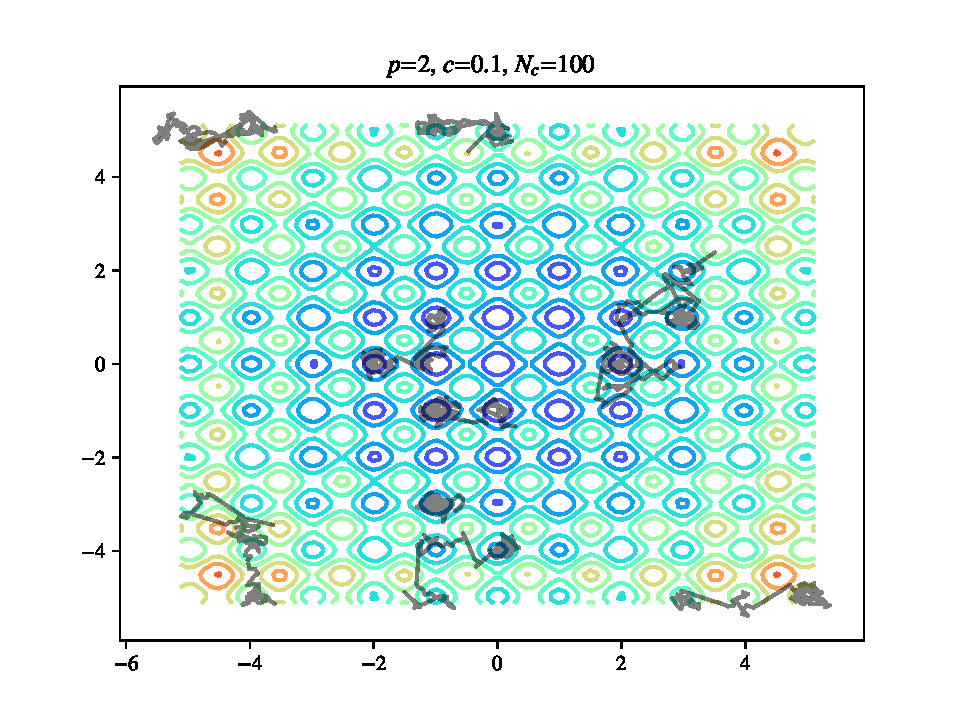
\includegraphics[scale=0.3]{assets/rastrigin_theta}
    \end{center}
  \column{0.5\textwidth}
    \begin{itemize}
      \item Relatively inconsistent performance for a highly nonconvex function
    \end{itemize}
\end{columns}
\end{frame}

\begin{frame}
\frametitle{Algorithm for a Colony}
\begin{algorithmic}[1]
\For {\textcolor{gray}{$j \gets 1 \dots N_c $}}:
  \For {$i \gets 1 \dots S$}:
    \State \textcolor{gray}{$\phi \sim S^p$}
    \State \textcolor{gray}{$\theta_i \gets \theta_i + c_i \phi$}
    \While {\textcolor{gray}{$J(\theta_i + c_i \phi)$} $+ J_{cc}(\theta_i + c_i \phi)$ \textcolor{gray}{$< J(\theta_i) $} $+ J_{cc}(\theta_i)$}:
      \State \textcolor{gray}{$\theta_i \gets \theta_i + c_i \phi$}
    \EndWhile
  \EndFor
\EndFor
\end{algorithmic}
\begin{itemize}
  \item $\theta_i$: $i$th $p$-dimensional vector (randomly initialized)
  \item $S$: number of bacteria in the colony
  \item $c_i$: a step-size for bacterium $i$
  \item $J_cc$: cell-to-cell interactions
\end{itemize}
\end{frame}

\begin{frame}
\frametitle{$J_{cc}$ and swarming behaviour}
\begin{itemize}
  \item \textit{\textit{E. coli}} do social foraging
  \item Secrete a substance to indicate to attract nearby \textit{\textit{E. coli}} and encourage swarming and biofilm formation
  \item Strength of signal diffuses over space
  \item Also want to avoid crowding
  \item Use sum of two Gaussian functions to model this
\end{itemize}
\begin{align*}
J_{cc}(\theta) = \sum_{i=1}^S &-d_\text{attract} \exp \left( -w_\text{attract} (\theta - \theta_i)^T (\theta - \theta_i) \right) \\ &+ h_\text{repellant} \exp \left( -w_\text{repellant} (\theta - \theta_i)^T (\theta - \theta_i) \right)
\end{align*}
\end{frame}

\begin{frame}
\frametitle{$J_{cc}$ and swarming behaviour}
\begin{center}
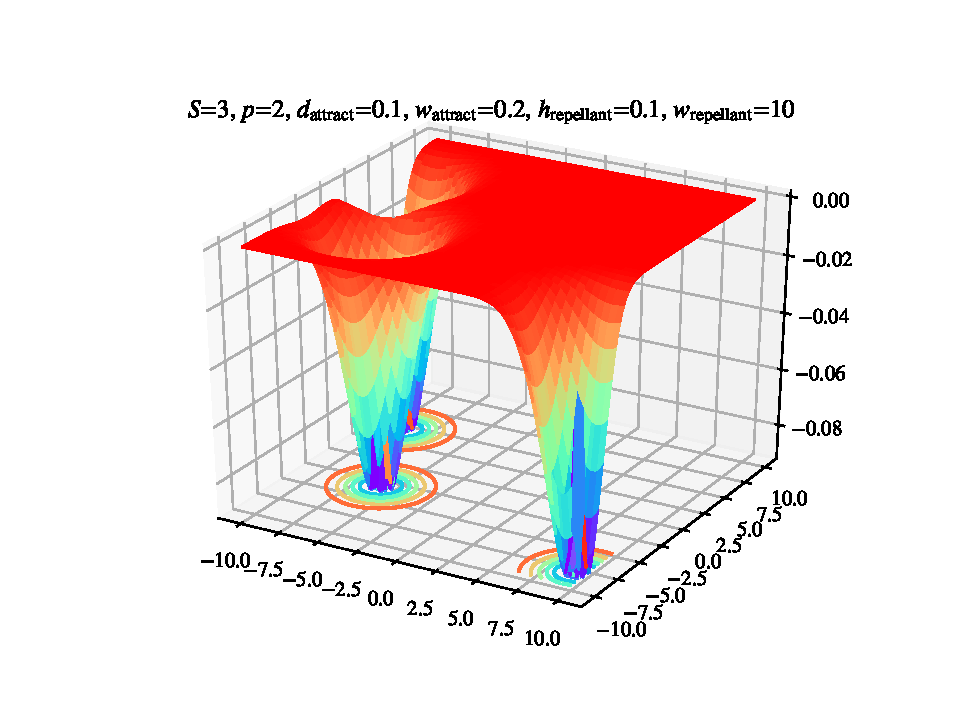
\includegraphics[scale=0.5]{assets/swarming}
\end{center}
\end{frame}

\begin{frame}
\frametitle{Results of Colony with Swarming}
\begin{columns}[T]
  \column{0.5\textwidth}
    \begin{center}
      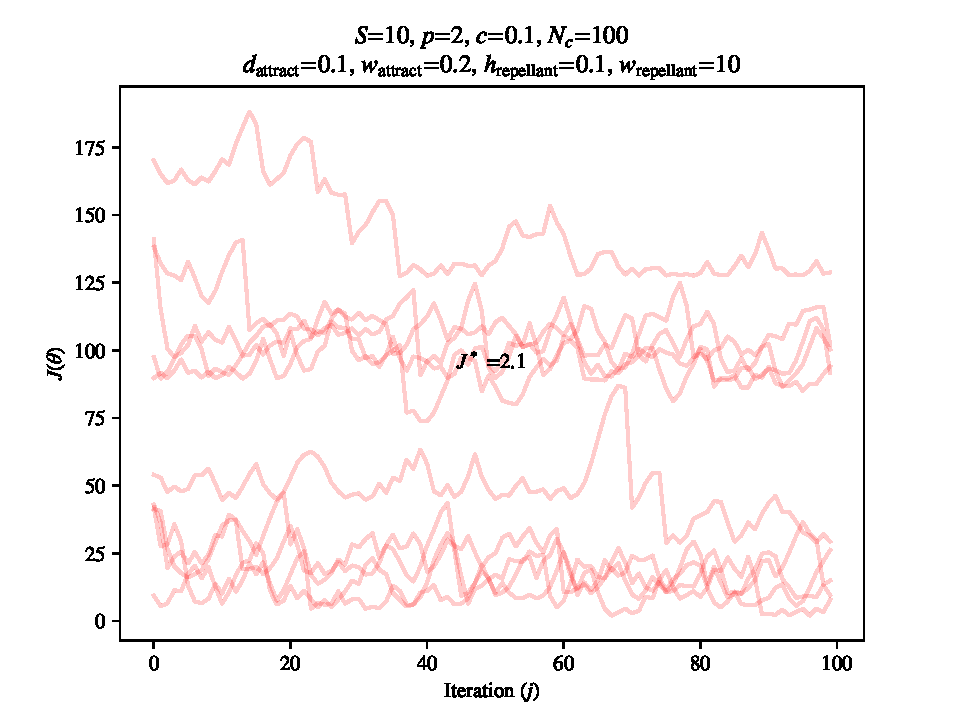
\includegraphics[scale=0.3]{assets/rastrigin_colony_J}
      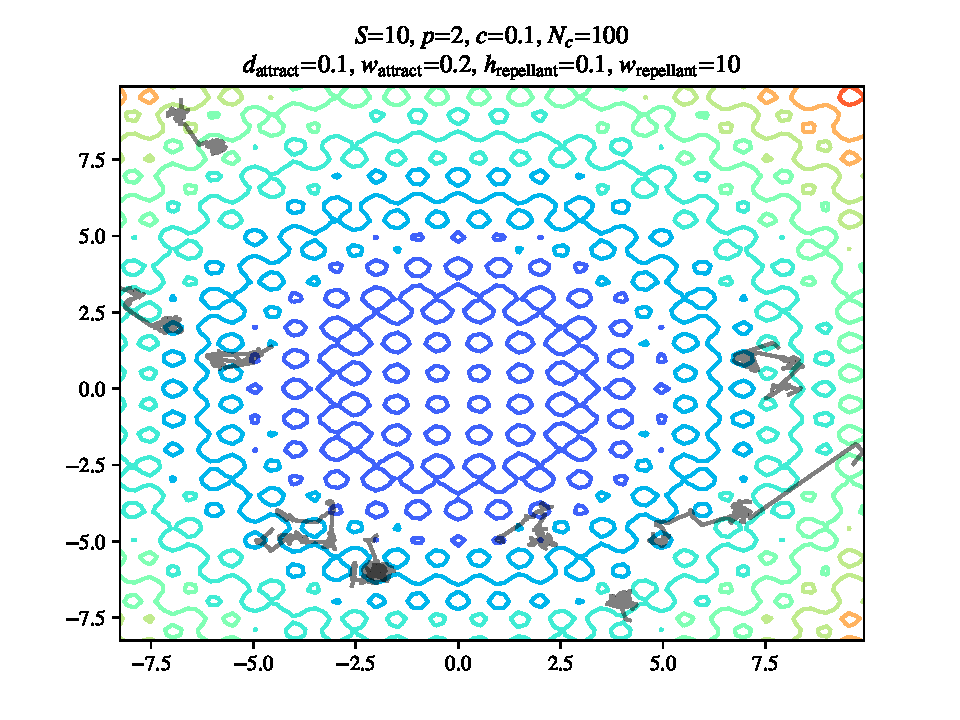
\includegraphics[scale=0.3]{assets/rastrigin_colony_theta}
    \end{center}
  \column{0.5\textwidth}
    \begin{itemize}
      \item Still relatively inconsistent performance for a highly nonconvex function
      \item But wait... What if the problem is just the hyperparameters?
    \end{itemize}
\end{columns}
\end{frame}

\begin{frame}
\frametitle{Results of Colony with Swarming}
\begin{columns}[T]
  \column{0.5\textwidth}
    \begin{center}
      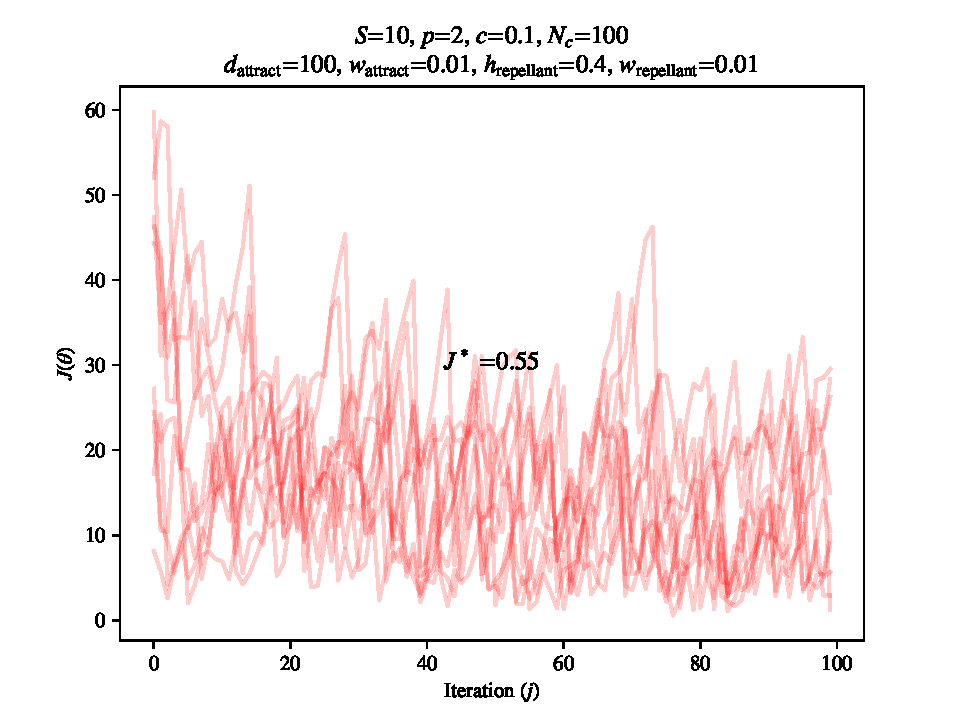
\includegraphics[scale=0.3]{assets/rastrigin_colony_tuned_J}
      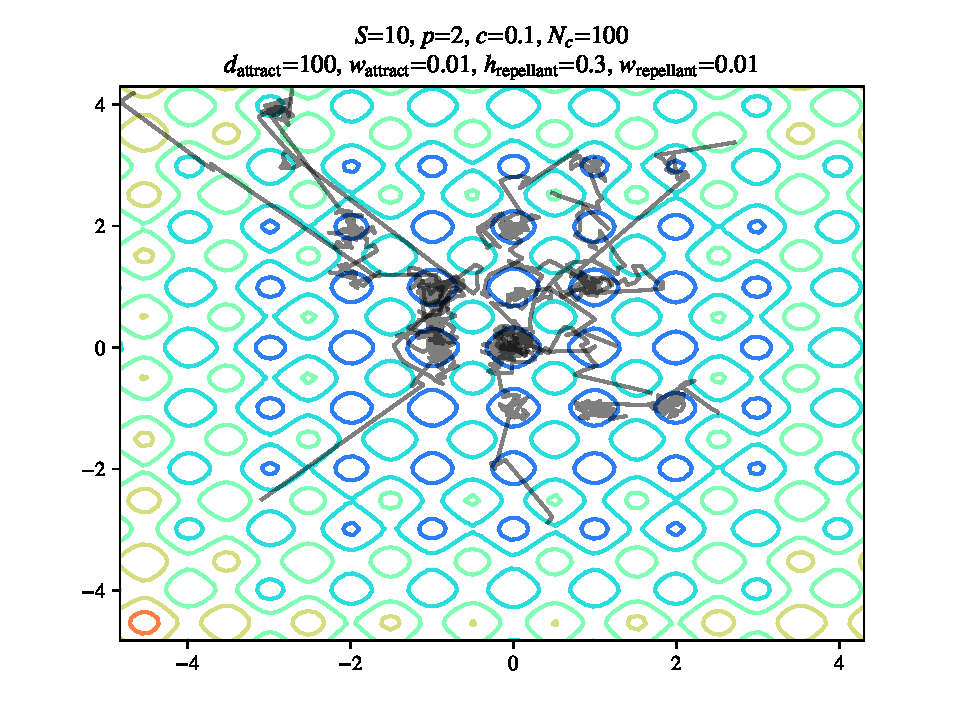
\includegraphics[scale=0.3]{assets/rastrigin_colony_tuned_theta}
    \end{center}
  \column{0.5\textwidth}
    \begin{itemize}
      \item<1-> By trying out different combinations of hyperparameters we can improve overall performance
      \item<1-> Here we increased the depth and width of attraction as well as the depth and width of repellance to increase "global" behaviour
      \item<2-> Important to know scale of $J$ relative to scale of $J_{cc}$ for tradeoff
      \begin{itemize}
        \item<2-> Can think of this like hyperparameters $c_1$ and $c_2$ for PSO
      \end{itemize}
    \end{itemize}
\end{columns}
\end{frame}

\begin{frame}
\frametitle{Comparing $J_{cc}$}
\begin{columns}[T]
  \column{0.5\textwidth}
  \begin{center}
    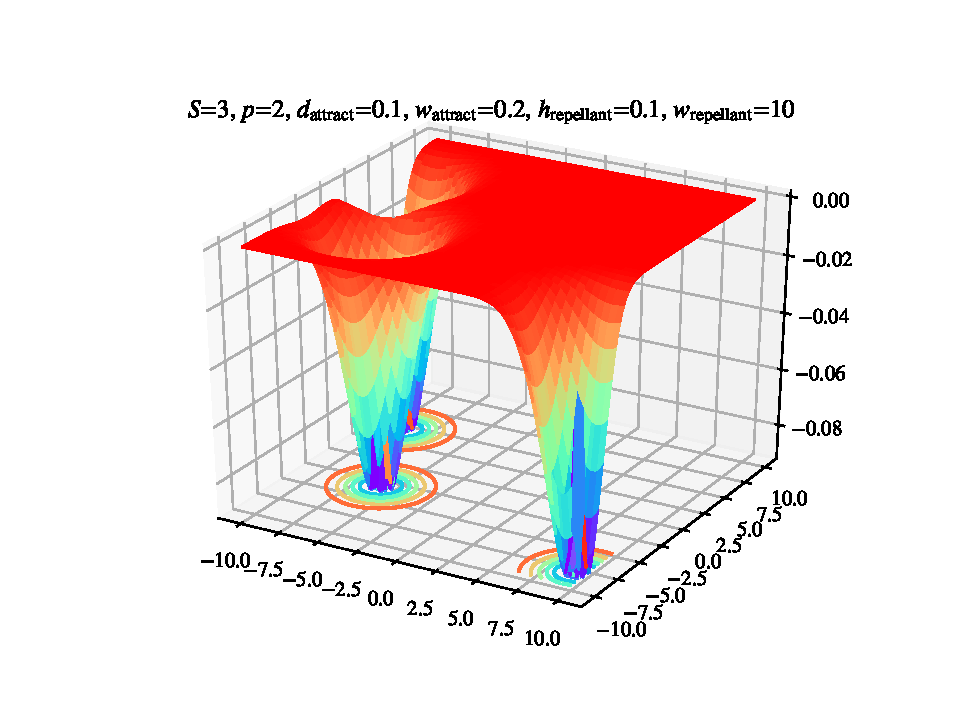
\includegraphics[scale=0.4]{assets/swarming}
  \end{center}
  \column{0.5\textwidth}
  \begin{center}
    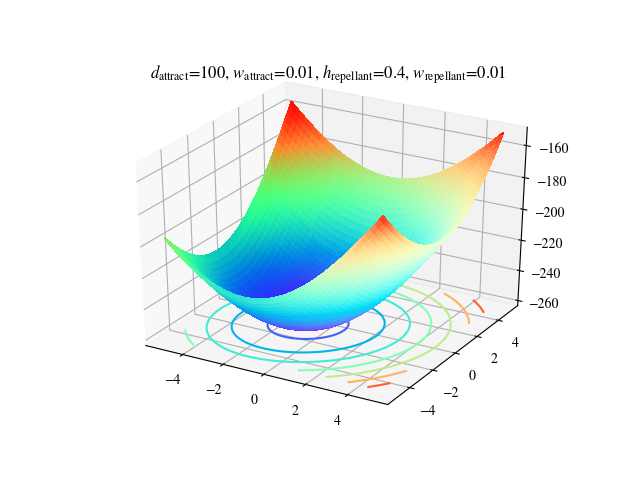
\includegraphics[scale=0.4]{assets/swarming_tuned}
  \end{center}
\end{columns}
\end{frame}

\begin{frame}
\frametitle{\textit{E. coli} reproduction}
\begin{itemize}
  \item<1-> \textit{E. coli} ``reproduce'' via
  \begin{enumerate}
    \item<1-> \textbf{Binary fission}: essentially creating a clone
    \item<1-> \textbf{Horizontal Translation}: merging genetic material with others
  \end{enumerate}
  \item<2-> Algorithm designed to mimic binary fission
  \begin{itemize}
    \item<2-> More fit individuals more likely to survive
    \item<2-> Less fit individuals more likely to die
  \end{itemize}
  \item<3-> Horizontal translation \text{could} be incorporated (like a genetic algorithm)
\end{itemize}
\end{frame}

\begin{frame}
\frametitle{Algorithm for a Reproducing Colony}
\begin{algorithmic}[1]
\For {$k \gets 1 \dots N_{re}$}:
  \For {\textcolor{gray}{$j \gets 1 \dots N_c $}}:
    \For {\textcolor{gray}{$i \gets 1 \dots S$}}:
      \State \textcolor{gray}{$\phi \sim S^p$}
      \State \textcolor{gray}{$\theta_i \gets \theta_i + c_i \phi$}
      \While {\textcolor{gray}{$J(\theta_i + c_i \phi) + J_{cc}(\theta_i + c_i \phi) < J(\theta_i) + J_{cc}(\theta_i)$}}:
        \State \textcolor{gray}{$\theta_i \gets \theta_i + c_i \phi$}
      \EndWhile
    \EndFor
  \EndFor
  \State delete worst $S/2$ and reproduce best $S/2$
\EndFor
\end{algorithmic}
\begin{itemize}
  \item $N_{re}$: number of reproduction steps
\end{itemize}
\end{frame}

\begin{frame}
\frametitle{Results of Reproducing Colony}
\begin{columns}[T]
  \column{0.5\textwidth}
    \begin{center}
      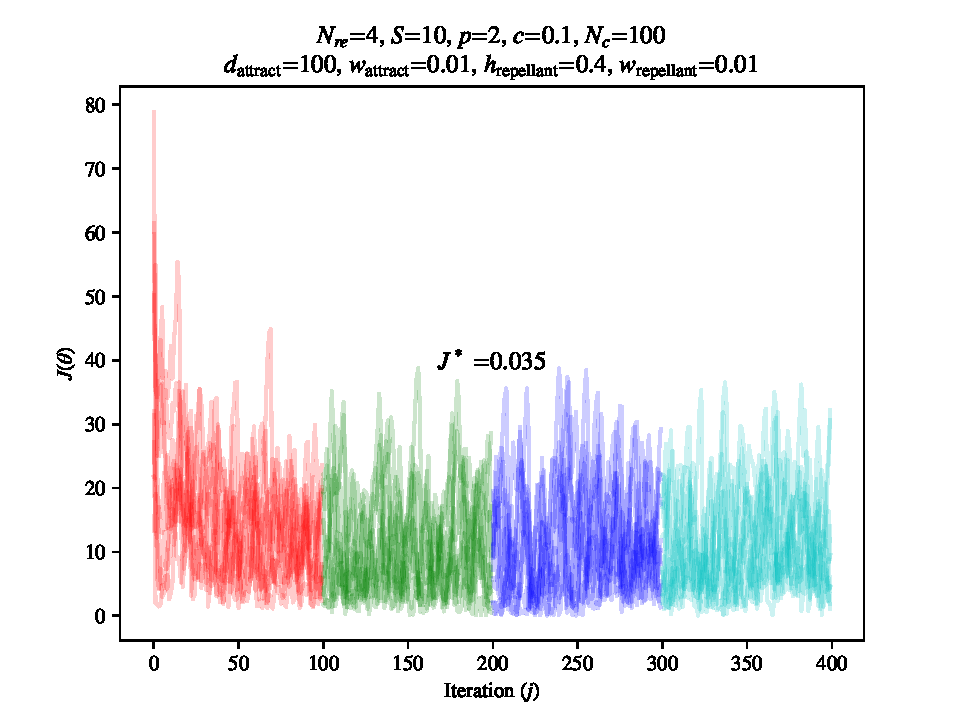
\includegraphics[scale=0.3]{assets/rastrigin_colony_re_J}
      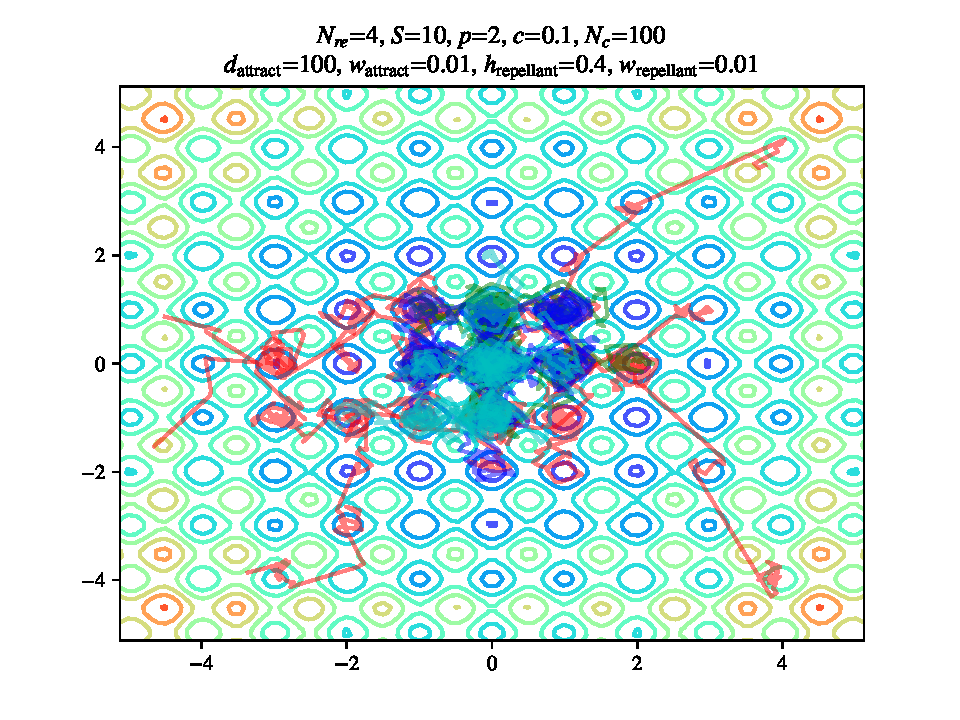
\includegraphics[scale=0.3]{assets/rastrigin_colony_re_theta}
    \end{center}
  \column{0.5\textwidth}
  \begin{itemize}
    \item<1-> Individuals with higher values of $J$ killed off
    \item<2-> Individuals with lower values of $J$ duplicated
    \begin{itemize}
      \item<2-> Ideally move away due to repellance
    \end{itemize}
    \item<3-> Idea is to encourage searching in space nearby ``best'' individuals
    \item<4-> If repellance isn't high enough then repeated iterations of evolution can concentrate colony in local minimum
  \end{itemize}
\end{columns}
\end{frame}

\begin{frame}
\frametitle{Does Reproduction Help?}
\begin{columns}[T]
  \column{0.5\textwidth}
    \begin{center}
      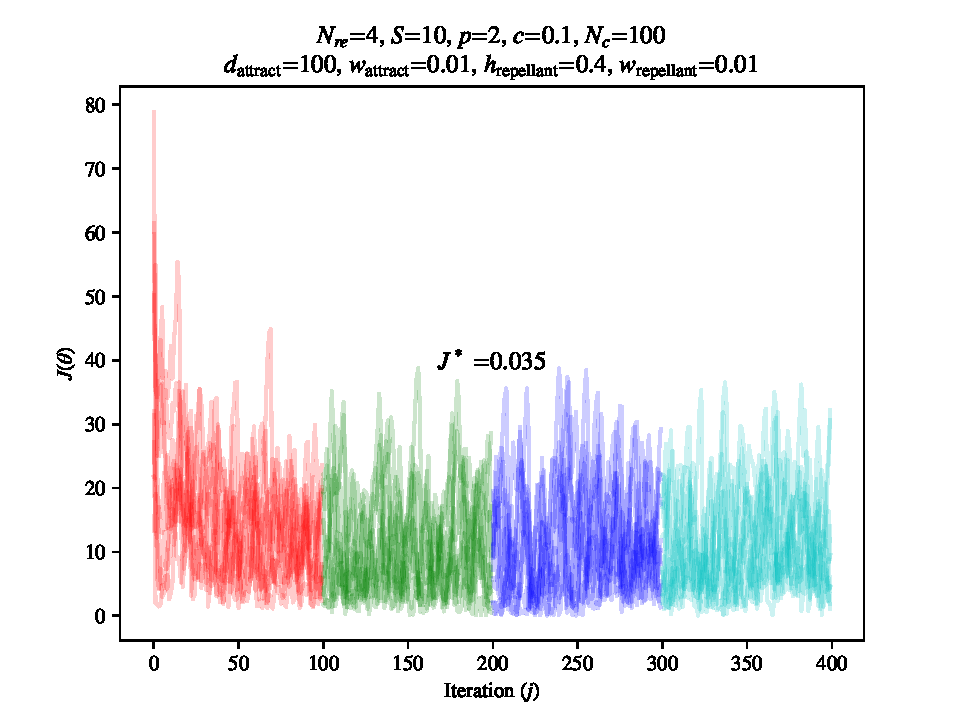
\includegraphics[scale=0.3]{assets/rastrigin_colony_re_J}
      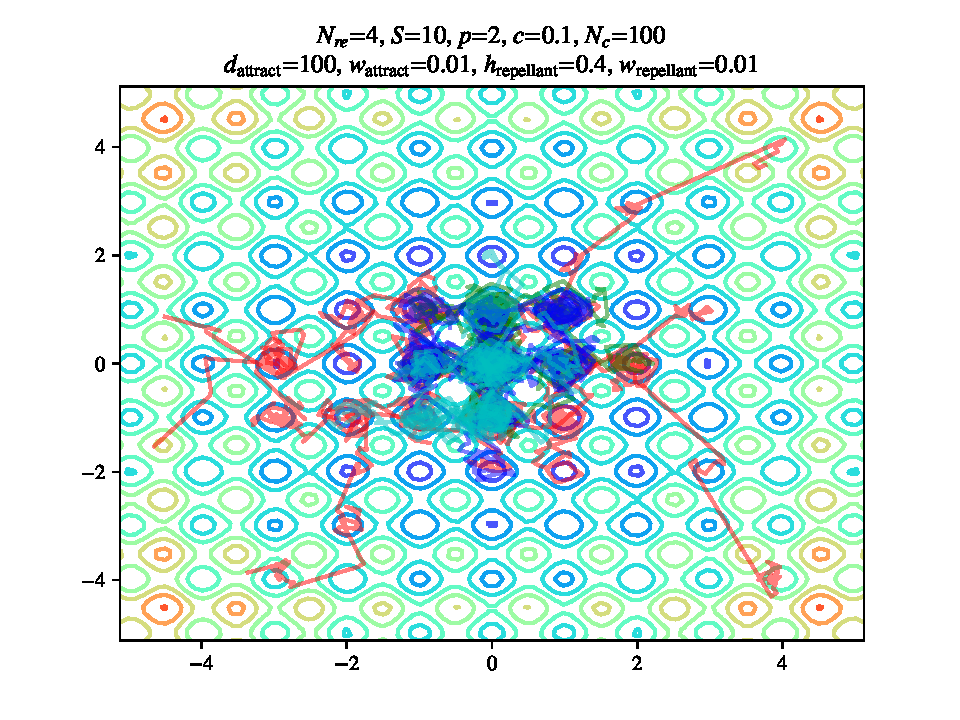
\includegraphics[scale=0.3]{assets/rastrigin_colony_re_theta}
    \end{center}
  \column{0.5\textwidth}
  \begin{center}
    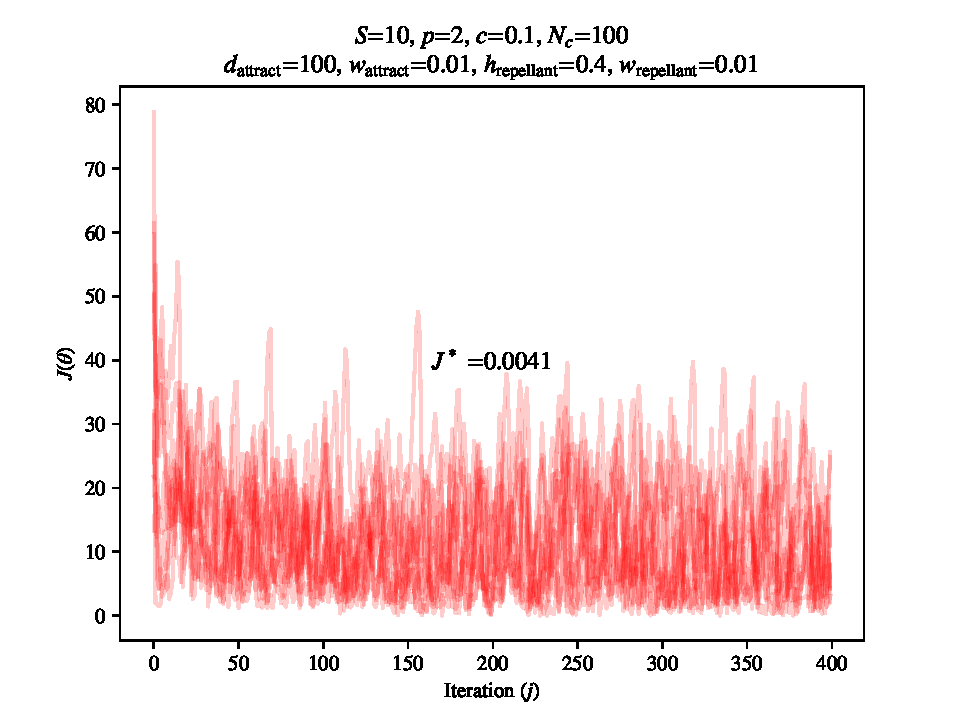
\includegraphics[scale=0.3]{assets/rastrigin_colony_400_J}
    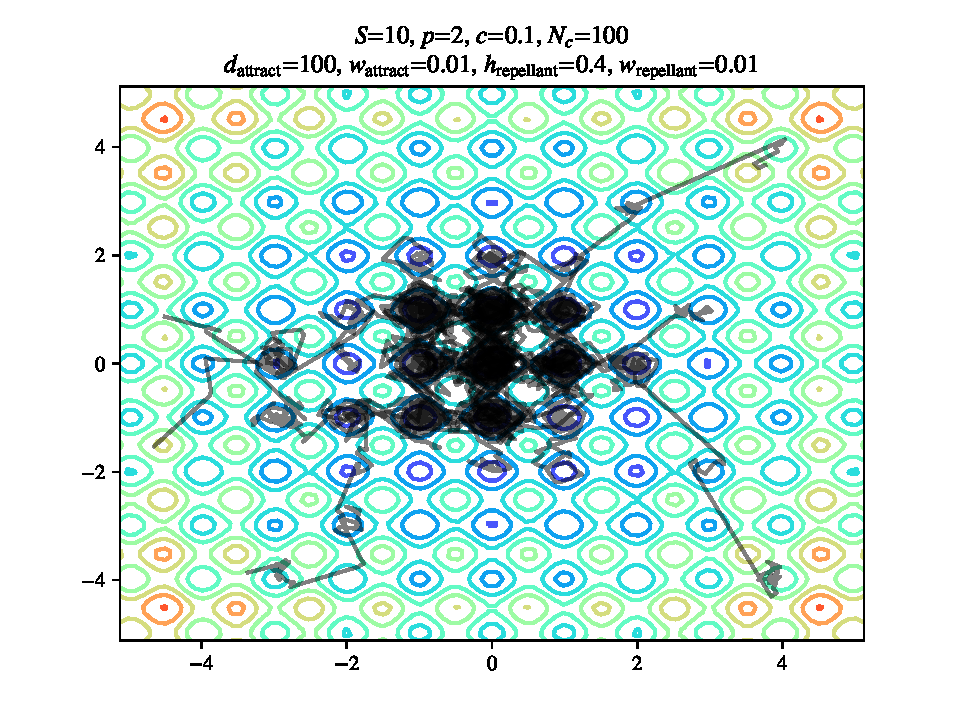
\includegraphics[scale=0.3]{assets/rastrigin_colony_400_theta}
  \end{center}
\end{columns}
\end{frame}

\begin{frame}
\frametitle{Elimination-Dispersal Events}
\begin{columns}[T]
\column{0.5\textwidth}
\begin{center}
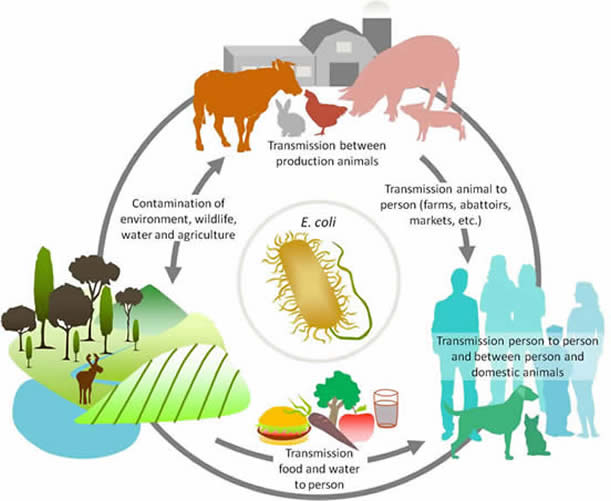
\includegraphics[scale=0.25]{assets/transmission.jpg}
\end{center}
\column{0.5\textwidth}
\begin{itemize}
  \item<1-> Over time, random events disperse populations of \textit{E. coli}
  \begin{itemize}
    \item<1-> Water, animal activity, human intervention
  \end{itemize}
  \item<2-> May destroy chemotactic progress
  \begin{itemize}
    \item<2-> But may also bring \textit{E. coli} to good food sources
  \end{itemize}
  \item<3-> For optimization, this is a method to prevent stagnation and move out from local minima
\end{itemize}
\end{columns}

\end{frame}

\begin{frame}
\frametitle{Algorithm for a Dispersing Colony}
\begin{algorithmic}[1]
\For {$l \gets 1 \dots N_{ed}$}:
  \For {\textcolor{gray}{$k \gets 1 \dots N_{re}$}}:
    \For {\textcolor{gray}{$j \gets 1 \dots N_c $}}:
      \For {\textcolor{gray}{$i \gets 1 \dots S$}}:
        \State \textcolor{gray}{$\phi \sim S^p$}
        \State \textcolor{gray}{$\theta_i \gets \theta_i + c_i \phi$}
        \While {\textcolor{gray}{$J(\theta_i + c_i \phi) + J_{cc}(\theta_i + c_i \phi) < J(\theta_i) + J_{cc}(\theta_i)$}}:
          \State \textcolor{gray}{$\theta_i \gets \theta_i + c_i \phi$}
        \EndWhile
      \EndFor
    \EndFor
    \State \textcolor{gray}{delete worst $S/2$ and reproduce best $S/2$}
  \EndFor
  \For {$i \gets 1 \dots S$}:
    \If {$\epsilon \sim \mathcal{U}(0, 1) < p_{ed}$}:
      \State $\theta_i \sim d^0(\theta)$
    \EndIf
  \EndFor
\EndFor
\end{algorithmic}
\begin{itemize}
  \item $N_{ed}$: number of elimination-dispersal events
  \item $p_{ed}$: probabilty of a single elimination-dispersal event
  \item $d^0(\theta)$: initial distribution of $\theta$
\end{itemize}
\end{frame}

\begin{frame}
\frametitle{Does Elimination-Dispersal Help?}
\begin{columns}[T]
  \column{0.5\textwidth}
    \begin{center}
      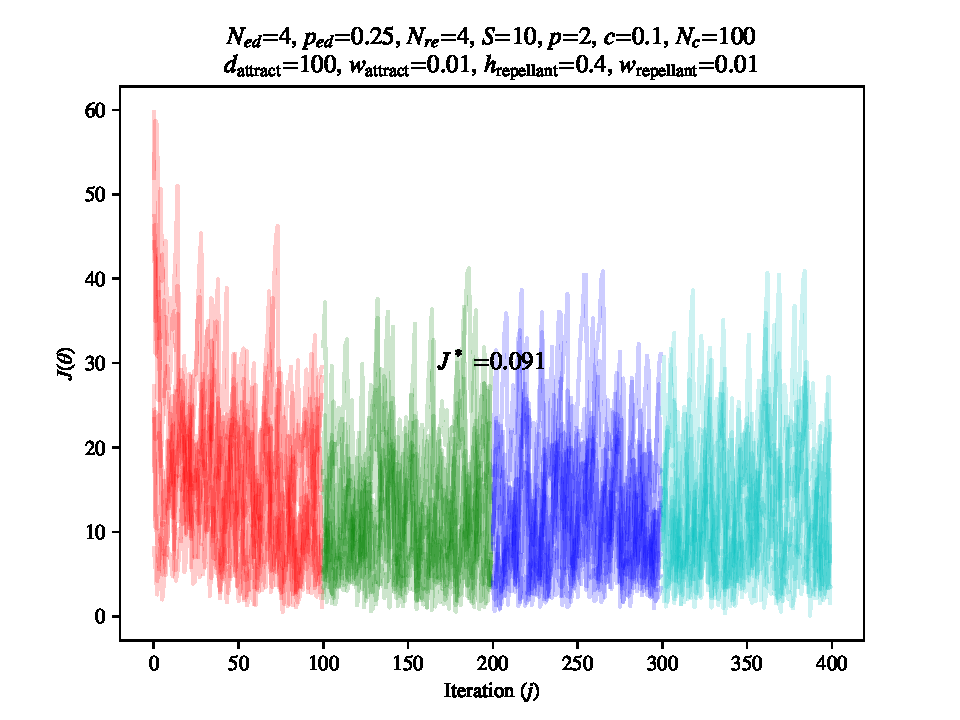
\includegraphics[scale=0.3]{assets/rastrigin_colony_ed_0_J}
      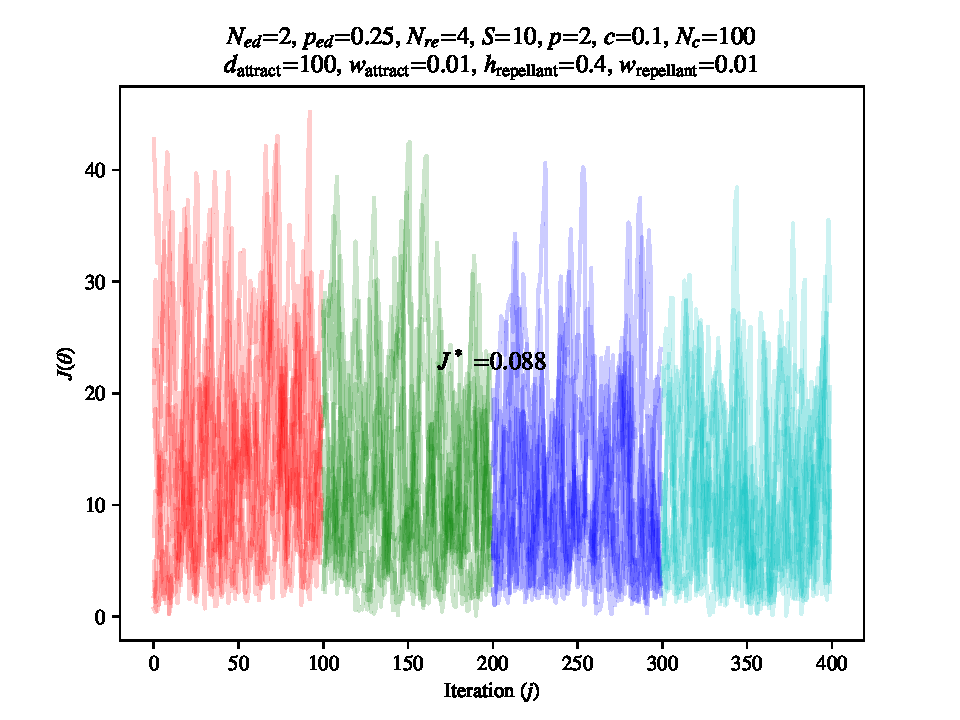
\includegraphics[scale=0.3]{assets/rastrigin_colony_ed_1_J}
    \end{center}
  \column{0.5\textwidth}
  \begin{center}
    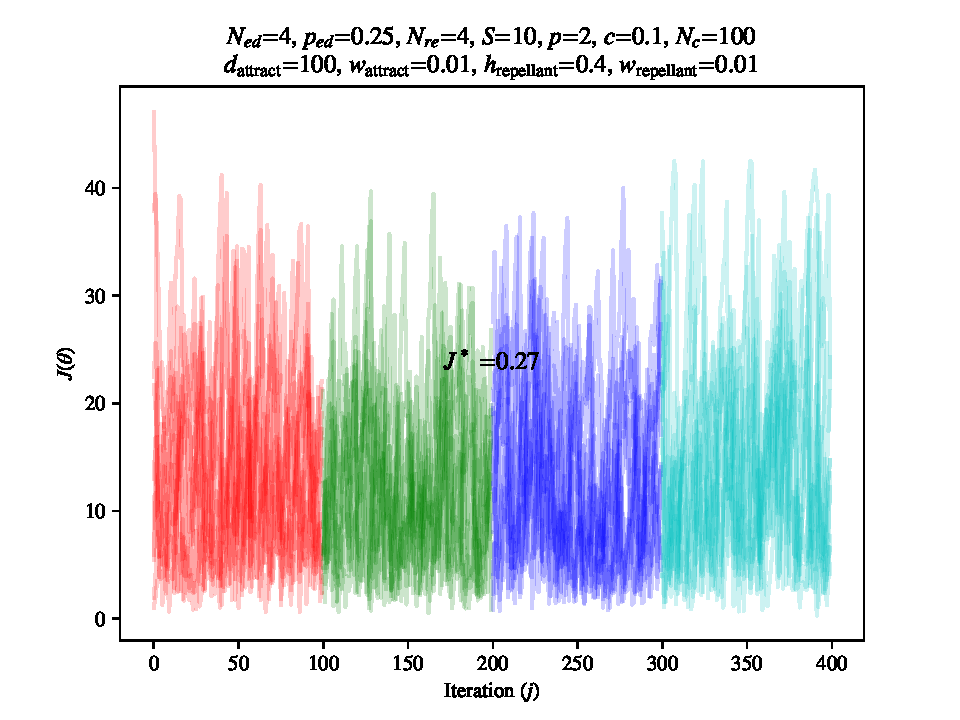
\includegraphics[scale=0.3]{assets/rastrigin_colony_ed_2_J}
    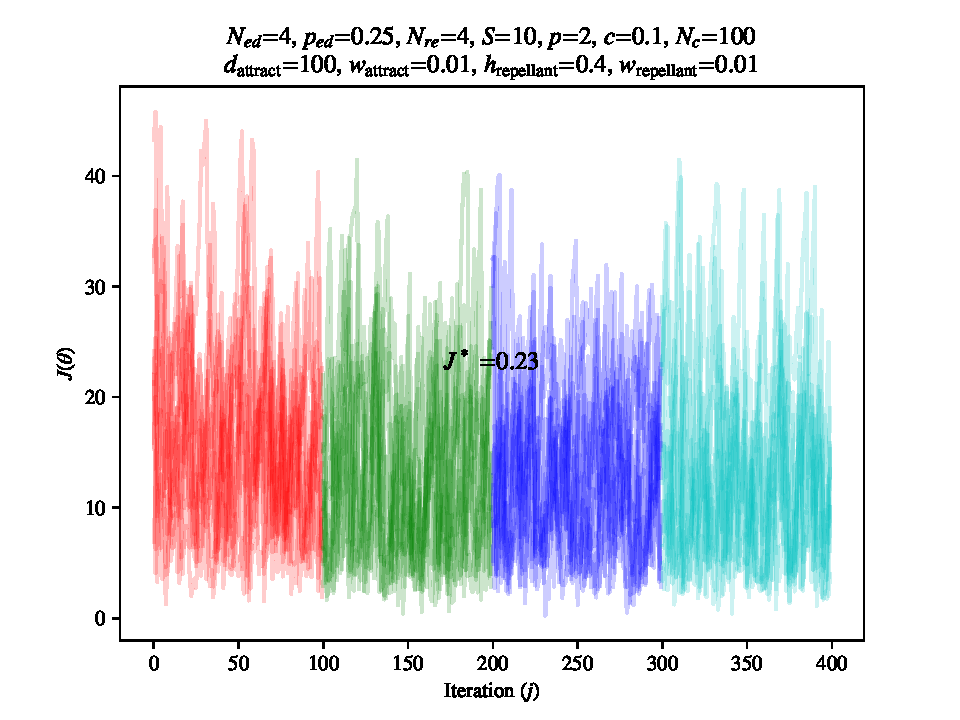
\includegraphics[scale=0.3]{assets/rastrigin_colony_ed_3_J}
  \end{center}
\end{columns}
\end{frame}

\begin{frame}
\frametitle{Caveats}
\begin{itemize}
  \item<1-> This is only a single application:
  \begin{itemize}
    \item<1-> A single highly nonconvex function
    \item<1-> Should try out other loss functions and applications (see post-presentation slides)
  \end{itemize}
  \item<2-> Chose a single seed arbitrarily to run experiments:
  \begin{itemize}
    \item<2-> Results could vary if a different seed was chosen
  \end{itemize}
  \item<3-> Hyperparameters were chosen by trying a few random combinations
  \begin{itemize}
    \item<3-> Tried to avoid ``overfitting'' hyperparameters (abuse of terminology)
  \end{itemize}
\end{itemize}
\end{frame}

\section{Discussion}

\begin{frame}
\frametitle{Is this a good optimization algorithm?}
\begin{itemize}
  \item<1-> We don't know. The authors don't compare to any existing methods.
  \item<2-> The author draws a comparison to genetic algorithms (GAs) since both are hill-climbing algorithms, but asserts that they are really different algorithms \textbf{based on their biological inspiration}
  \begin{itemize}
    \item<2-> Is this really enough to make it a novel algorithm?
  \end{itemize}
  \item<3-> The method is also suspiciously similar to partical swarm optimization
  \begin{itemize}
    \item<4-> Combines local and global information with stochastic hill-climbing algorithm
    \item<4-> The authors never mention this despite the popularity of PSOs (this paper publish 7 years later)
    \item<5-> (Ask me about the comparison I did afterwards!)
  \end{itemize}
\end{itemize}
\end{frame}

\begin{frame}
\frametitle{Is this a good optimization algorithm?}
\begin{itemize}
  \item<1-> However, this algorithm is \textbf{gradient-free}
  \begin{itemize}
    \item<2-> We can minimize functions that we may not have access to the gradient for (or it may not exist)
    \item<2-> For example (from the paper) fitting model parameters for dynamic control problem
    \item<2-> Or for example fitting the parameters of a neural network to perform a task
  \end{itemize}
  \item<3-> It can also explore the search space beyond the initial distribution $d^0(\theta)$ in case we do not know where the optimal value $\theta^*$ lies
\end{itemize}
\end{frame}

\begin{frame}
\frametitle{Is this a good model of \textit{E. coli}?}
\begin{itemize}
  \item<2-> We don't know. The authors don't compare to any ecological data.
\end{itemize}
\end{frame}


\begin{frame}
\frametitle{Is this a good model of \textit{E. coli}?}
Some important limitations from the authors:
\begin{itemize}
  \item<1> Ignore characteristics of actual biological processes in favor of simplicity and capturing the essence of chemotactic hill-climbing and swarming
  \item<2> Ignore characteristics of the chemical medium and  assume that consumption does not affect the nutrient surface
  \item<3> They assume a constant population size, even if there are many nutrients and generations
  \item<4> They assume that the cells respond to nutrients in the environment in the same way that they respond to ones released by other cells for the purpose of signaling the desire to swarm
\end{itemize}
\end{frame}

\begin{frame}
\frametitle{Is this a good paper?}
\begin{center}
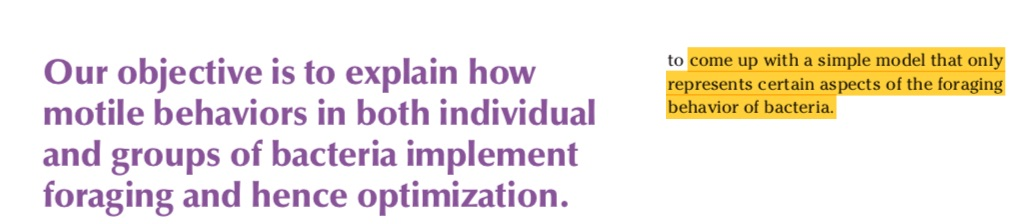
\includegraphics[scale=0.3]{assets/yikes}
\end{center}
\end{frame}

\begin{frame}
\frametitle{Is this a good paper?}
\begin{itemize}
  \item<1-> A significant portion of the paper is dedicated to discussing biology and foraging
  \begin{itemize}
    \item <1-> This information is later thrown away during development of the algorithm
  \end{itemize}
  \item<2-> It is not clear if the goal is create a simulation of \textit{E. coli} foraging behaviour or to create another biologically-inspired optimization algorithm
\end{itemize}
\end{frame}

\begin{frame}
\frametitle{Discussion}
\end{frame}

\begin{frame}
\frametitle{Lessons Learned}
\begin{itemize}
  \item<1-> As with any stochastic algorithm, \textbf{your random seed matters}
  \begin{itemize}
    \item<1-> I often got wildly different results for different initial seeds
    \item<1-> This might be alleviated by having larger populations, but that comes at a computational cost
  \end{itemize}
  \item<2-> As with any algorithm with lots of hyperparameters, tuning hyperparameters can be hard
  \begin{itemize}
    \item<2-> For a fixed seed with a grid search you may find good hyperparameters
    \item<2-> But those hyperparameters may not be robust so seed changes
  \end{itemize}
  \item<3-> As with any algorithm, trying a single loss function is not usually sufficient
  \begin{itemize}
    \item<3-> I chose rastrigin specifically for its difficulty
    \item<3-> However, you run the risk of ``overfitting'' your algorithm and hyperparameters to a single problem
  \end{itemize}
\end{itemize}
\end{frame}

\begin{frame}
\frametitle{Comparison to PSO}
\begin{itemize}
  \item Bacterial foraging method:
  \begin{itemize}
    \item   At least $N_{ed} \times N_{re} \times S \times N_c$ values of $\theta$ seen
  \end{itemize}
  \item PSO: $N \times \text{iter}$ values of $\theta$ seen
  \begin{itemize}
    \item PSO strongest with large $N$, so presume $\text{iter} \equiv N_c$
    \item Then $N = N_{ed} \times N_{re} \times S$
  \end{itemize}
\end{itemize}
\end{frame}

\begin{frame}
\frametitle{Comparison to PSO}
\begin{columns}[T]
  \column{0.5\textwidth}
    \begin{center}
      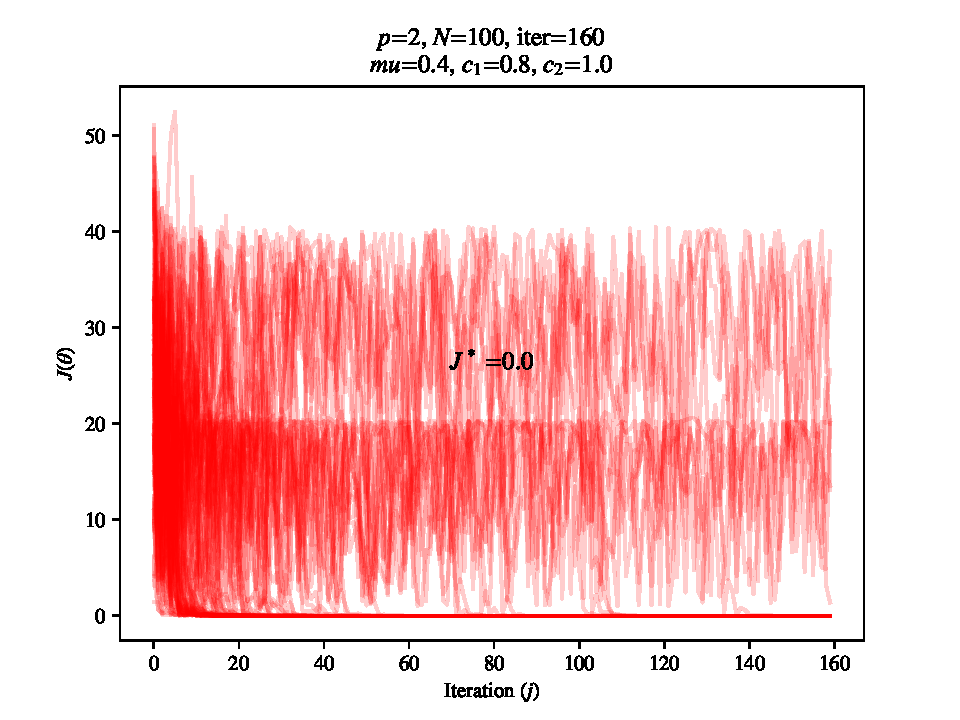
\includegraphics[scale=0.3]{assets/pso_J}
      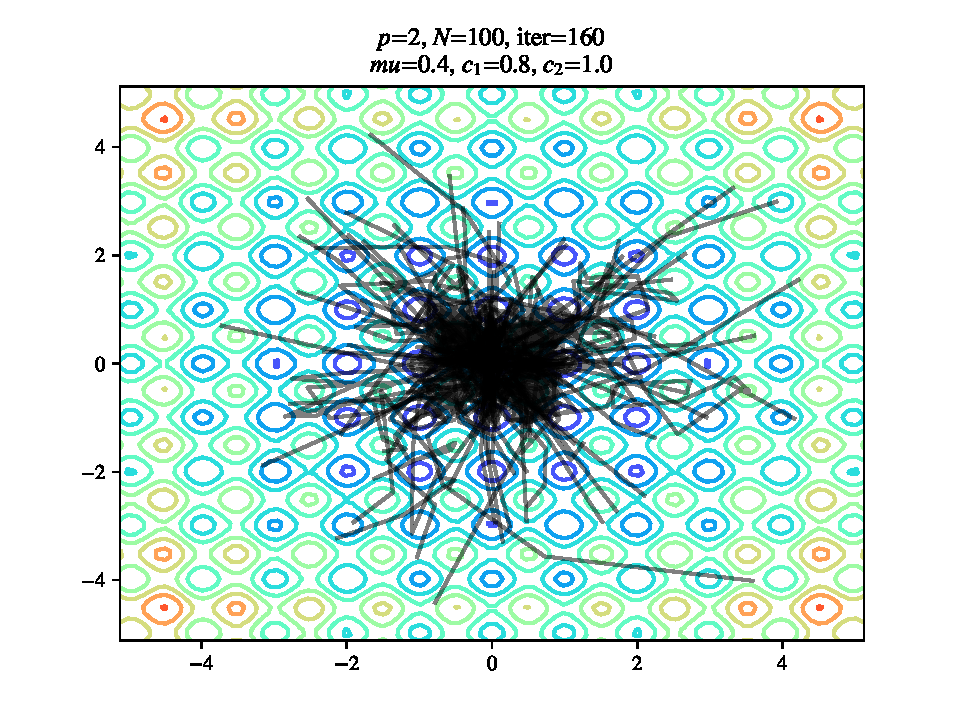
\includegraphics[scale=0.3]{assets/pso_theta}
    \end{center}
  \column{0.5\textwidth}
  \begin{center}
    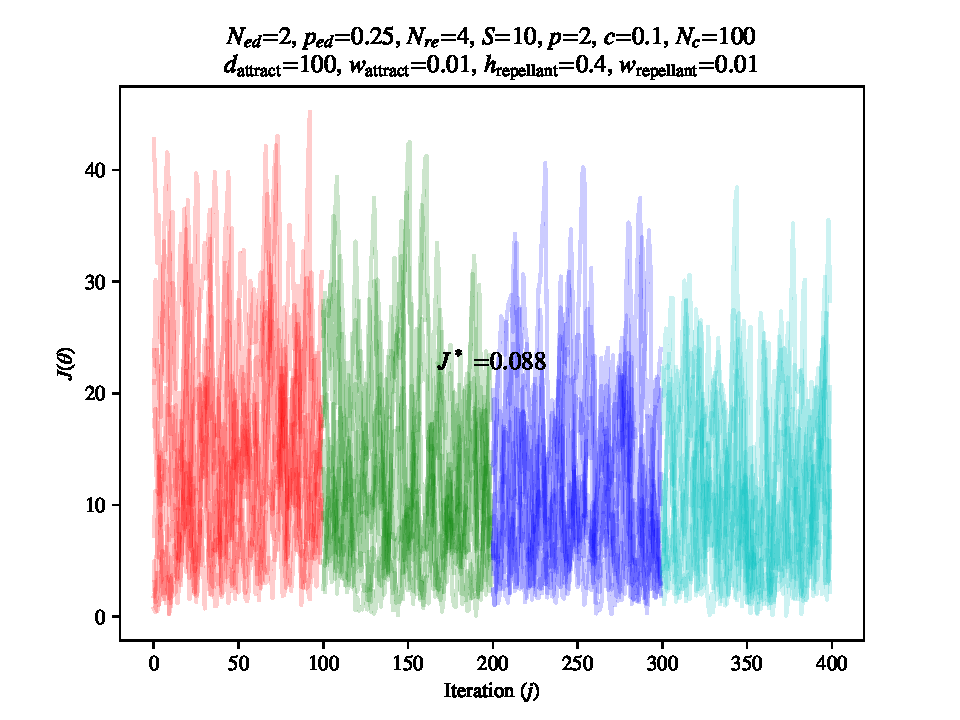
\includegraphics[scale=0.3]{assets/rastrigin_colony_ed_1_J}
    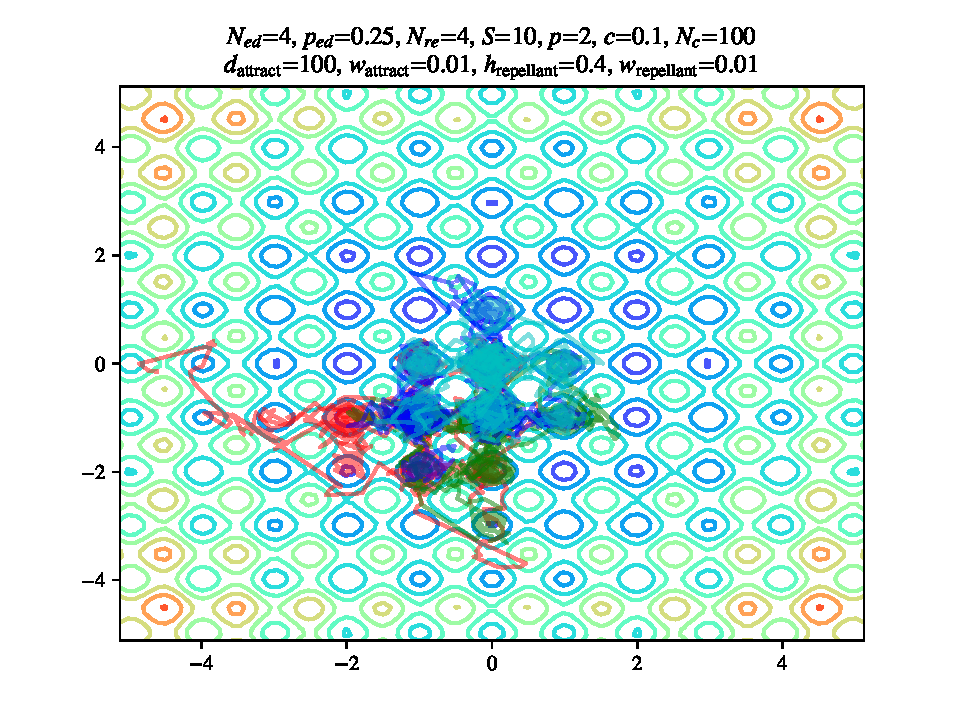
\includegraphics[scale=0.3]{assets/rastrigin_colony_ed_1_theta}
  \end{center}
\end{columns}
\end{frame}

\end{document}
